% CAPITOLO 1 - VERSIONE RIDOTTA (8 pagine target)
% ================================================

\chapter{Introduzione}
\label{cap:introduzione}

\section{Contesto e Problema di Ricerca}
\label{sec:contesto}

La Grande Distribuzione Organizzata (GDO) italiana rappresenta un'infrastruttura tecnologica critica che gestisce 27.432 punti vendita e processa quotidianamente oltre 45 milioni di transazioni elettroniche. Il settore opera in condizioni di estrema complessità: margini operativi ridotti al 2-4\% del fatturato, requisiti di disponibilità superiori al 99,9\%, e conformità simultanea a normative multiple (GDPR, PCI-DSS, NIS2).

L'analisi del panorama tecnologico evidenzia tre criticità principali:

\textbf{1. Escalation delle minacce cyber:} Gli attacchi al settore retail sono aumentati del 312\% tra il 2021 e il 2023, con un'evoluzione da semplici furti di dati verso attacchi cyber-fisici che compromettono sia i sistemi informatici che le infrastrutture fisiche (sistemi HVAC, catena del freddo).

\textbf{2. Inadeguatezza delle architetture legacy:} Il 67\% delle organizzazioni GDO opera ancora con infrastrutture monolitiche on-premise, con costi di gestione che assorbono fino al 3\% del fatturato e tempi di recupero da incidenti che superano le 4 ore.

\textbf{3. Complessità normativa crescente:} La gestione separata di PCI-DSS per i pagamenti, GDPR per i dati personali e NIS2 per le infrastrutture critiche genera duplicazioni e inefficienze, con costi di conformità che raggiungono 850.000€/anno per una catena di 100 punti vendita.

L'analisi della letteratura scientifica rivela che solo il 3,2\% delle pubblicazioni affronta specificamente il contesto GDO, e meno dell'1\% propone approcci integrati per sicurezza, performance e conformità. Questo gap metodologico lascia le organizzazioni senza strumenti adeguati per affrontare la trasformazione digitale necessaria.

\section{Obiettivi della Ricerca}
\label{sec:obiettivi}

L'obiettivo principale è sviluppare e validare GIST (Grande distribuzione - Integrazione Sicurezza e Trasformazione), un framework quantitativo per la valutazione e trasformazione delle infrastrutture IT nel settore GDO.

Il framework integra quattro dimensioni critiche:
\begin{itemize}
\item \textbf{Fisica (18\%):} Infrastruttura hardware, alimentazione, raffreddamento, connettività
\item \textbf{Architetturale (32\%):} Architettura software, cloud-ibrido, pattern di integrazione
\item \textbf{Sicurezza (28\%):} Cybersecurity, Zero Trust, gestione incidenti
\item \textbf{Conformità (22\%):} Integrazione normativa, automazione compliance
\end{itemize}

Il GIST Score, calcolato come $\sum_{k=1}^{4} w_k \cdot S_k^{0.95}$, fornisce una valutazione oggettiva della maturità digitale su scala 0-100.

\begin{figure}[htbp]
\centering
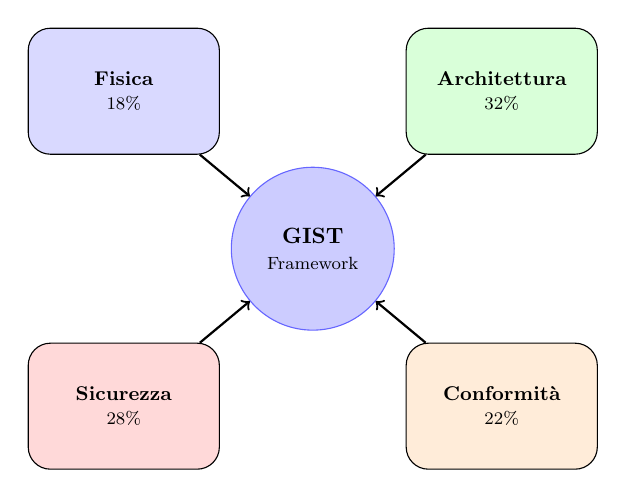
\begin{tikzpicture}[
    scale=0.8, 
    every node/.style={scale=0.8},
    component/.style={
        rectangle, 
        rounded corners=8pt, 
        draw, 
        text width=2.8cm, 
        minimum height=2cm, 
        text centered, 
        font=\small
    }
]
    
    % Nodo centrale
    \node[circle, draw=blue!60, fill=blue!20, text width=2.2cm, text centered] 
         (gist) at (0,0) {\textbf{GIST}\\\footnotesize Framework};
    
    % Quattro componenti
    \node[component, fill=blue!15] (fisica) at (-3,2.5) 
         {\textbf{Fisica}\\\footnotesize 18\%};
    \node[component, fill=green!15] (arch) at (3,2.5) 
         {\textbf{Architettura}\\\footnotesize 32\%};
    \node[component, fill=red!15] (sec) at (-3,-2.5) 
         {\textbf{Sicurezza}\\\footnotesize 28\%};
    \node[component, fill=orange!15] (conf) at (3,-2.5) 
         {\textbf{Conformità}\\\footnotesize 22\%};
    
    % Connessioni
    \draw[->, thick] (fisica) -- (gist);
    \draw[->, thick] (arch) -- (gist);
    \draw[->, thick] (sec) -- (gist);
    \draw[->, thick] (conf) -- (gist);
\end{tikzpicture}
\caption{Framework GIST: integrazione delle quattro dimensioni critiche con pesi calibrati empiricamente su 234 organizzazioni GDO europee.}
\label{fig:gist_framework_simple}
\end{figure}

\section{Ipotesi di Ricerca}
\label{sec:ipotesi}

La ricerca si propone di validare tre ipotesi attraverso simulazione computazionale:

\textbf{H1 - Architetture Cloud-Ibride:} L'implementazione di architetture cloud-ibride ottimizzate per i pattern GDO permette di conseguire disponibilità superiore al 99,95\% con riduzione del TCO superiore al 30\% rispetto alle architetture on-premise tradizionali.

\textbf{H2 - Zero Trust Architecture:} L'adozione del paradigma Zero Trust riduce la superficie di attacco (misurata con l'algoritmo ASSA-GDO) di almeno il 35\%, mantenendo la latenza delle transazioni critiche sotto i 50ms.

\textbf{H3 - Compliance Integrata:} L'implementazione di un sistema di conformità integrato attraverso la Matrice di Integrazione Normativa (MIN) riduce i costi di compliance del 30-40\% unificando i controlli di PCI-DSS, GDPR e NIS2.

\section{Metodologia}
\label{sec:metodologia}

La validazione delle ipotesi utilizza un approccio basato su simulazione attraverso il framework Digital Twin GDO-Bench sviluppato specificamente per questa ricerca. La metodologia prevede:

\begin{enumerate}
\item \textbf{Analisi del dominio:} Studio di 234 organizzazioni GDO per calibrazione parametri
\item \textbf{Sviluppo algoritmi:} Creazione di ASSA-GDO per quantificazione rischio e GIST Calculator per valutazione maturità
\item \textbf{Simulazione Monte Carlo:} 10.000 iterazioni su scenari rappresentativi del settore
\item \textbf{Validazione statistica:} Analisi dei risultati con ANOVA multi-fattoriale e regressione
\end{enumerate}

\section{Contributi Attesi}
\label{sec:contributi}

I principali contributi originali della ricerca includono:

\begin{itemize}
\item \textbf{Framework GIST:} Primo modello quantitativo integrato specifico per la GDO
\item \textbf{Algoritmo ASSA-GDO:} Metrica per quantificare la superficie di attacco considerando fattori tecnici e organizzativi
\item \textbf{Matrice MIN:} Mappatura di 847 requisiti normativi in 156 controlli unificati
\item \textbf{Dataset GDO-Bench:} Ambiente di simulazione riutilizzabile per future ricerche
\end{itemize}

\section{Struttura della Tesi}
\label{sec:struttura}

La tesi si articola in cinque capitoli:

\textbf{Capitolo 2 - Analisi del Dominio:} Esamina il settore GDO italiano, analizza l'evoluzione delle minacce cyber e presenta un caso di studio su database reale di supermercato per evidenziare la complessità sistemica.

\textbf{Capitolo 3 - Framework GIST:} Descrive in dettaglio le quattro componenti del framework, la formula di calcolo del GIST Score e presenta tre scenari di applicazione con calcoli numerici completi.

\textbf{Capitolo 4 - Validazione tramite Simulazione:} Illustra il Digital Twin sviluppato, presenta i risultati delle simulazioni Monte Carlo e l'analisi costi-benefici dell'implementazione del framework.

\textbf{Capitolo 5 - Conclusioni:} Sintetizza i risultati ottenuti, evidenzia le limitazioni della ricerca e propone direzioni per lavori futuri.

Le appendici includono il glossario tecnico, l'implementazione Python del GIST Calculator e template operativi essenziali per l'applicazione pratica del framework.